Les neuvièmes Rencontres Jeunes Chercheur·e·s en EIAH (RJC EIAH 2022) se sont tenues à l’Université de Lille du 9 au 11 mai 2022, succédant ainsi à la huitième édition (RJC EIAH, 2020) qui s’était déroulée exclusivement en ligne du fait de la situation sanitaire.  
Aussi, après deux années de mise à distance de la plupart des conférences et colloques, ces rencontres sont une occasion particulièrement importantes pour les jeunes chercheur·e·s de la communauté EIAH (Environnements Informatiques pour l’Apprentissage Humain) de pouvoir se rencontrer et échanger autour de leur travaux avec des pairs et des chercheur·e·s séniors. 

En effet, ces rencontres francophones, organisées tous les 2 ans sous l’égide de l’ATIEF (Association des Technologies de l'Information pour l'Éducation et la Formation) visent le développement de la communauté EIAH par la formation des jeunes chercheur.e.s issus des différentes disciplines inhérentes au domaine des EIAH et la diffusion de leurs travaux. 

\begin{figure}[!ht]
	\centering
	\includegraphics[width=0.8\textwidth]{Content/figures/carteComplete.png}
	\caption{Répartition géographique des publications}
	\label{f:repGeoPubli}
\end{figure}

L’édition 2022 a retenu l’attention de 30 jeunes chercheur.e.s qui ont soumis une contribution sous forme d’article de 6 pages pour 28 d’entre eux, et de poster de 2 pages pour deux autres. 
Chacune de ces communications ont été évaluées par 3 membres du comité de programme issus de différentes disciplines de l’Informatique et des Sciences Humaines et Sociales. À l’issue de cette phase d'évaluation, 19 propositions ont été acceptées sous la forme d’articles longs, et 10 ont été acceptées sous la forme d’un poster.  
Nous remercions le comité de programme pour la qualité  des relectures et les commentaires conséquents qui permettent l’amélioration des articles et posters proposés et des présentations lors de la conférence.

Les contributions proviennent essentiellement d’universités françaises, mais comptent également des travaux issus de Suisse (3) et du Maroc (1) (voir Figure \ref{f:repGeoPubli}). 
Les publications sont ainsi issues de 18 universités ou écoles différentes et de 14 laboratoires de recherches.

\begin{figure}[ht]
	\centering
	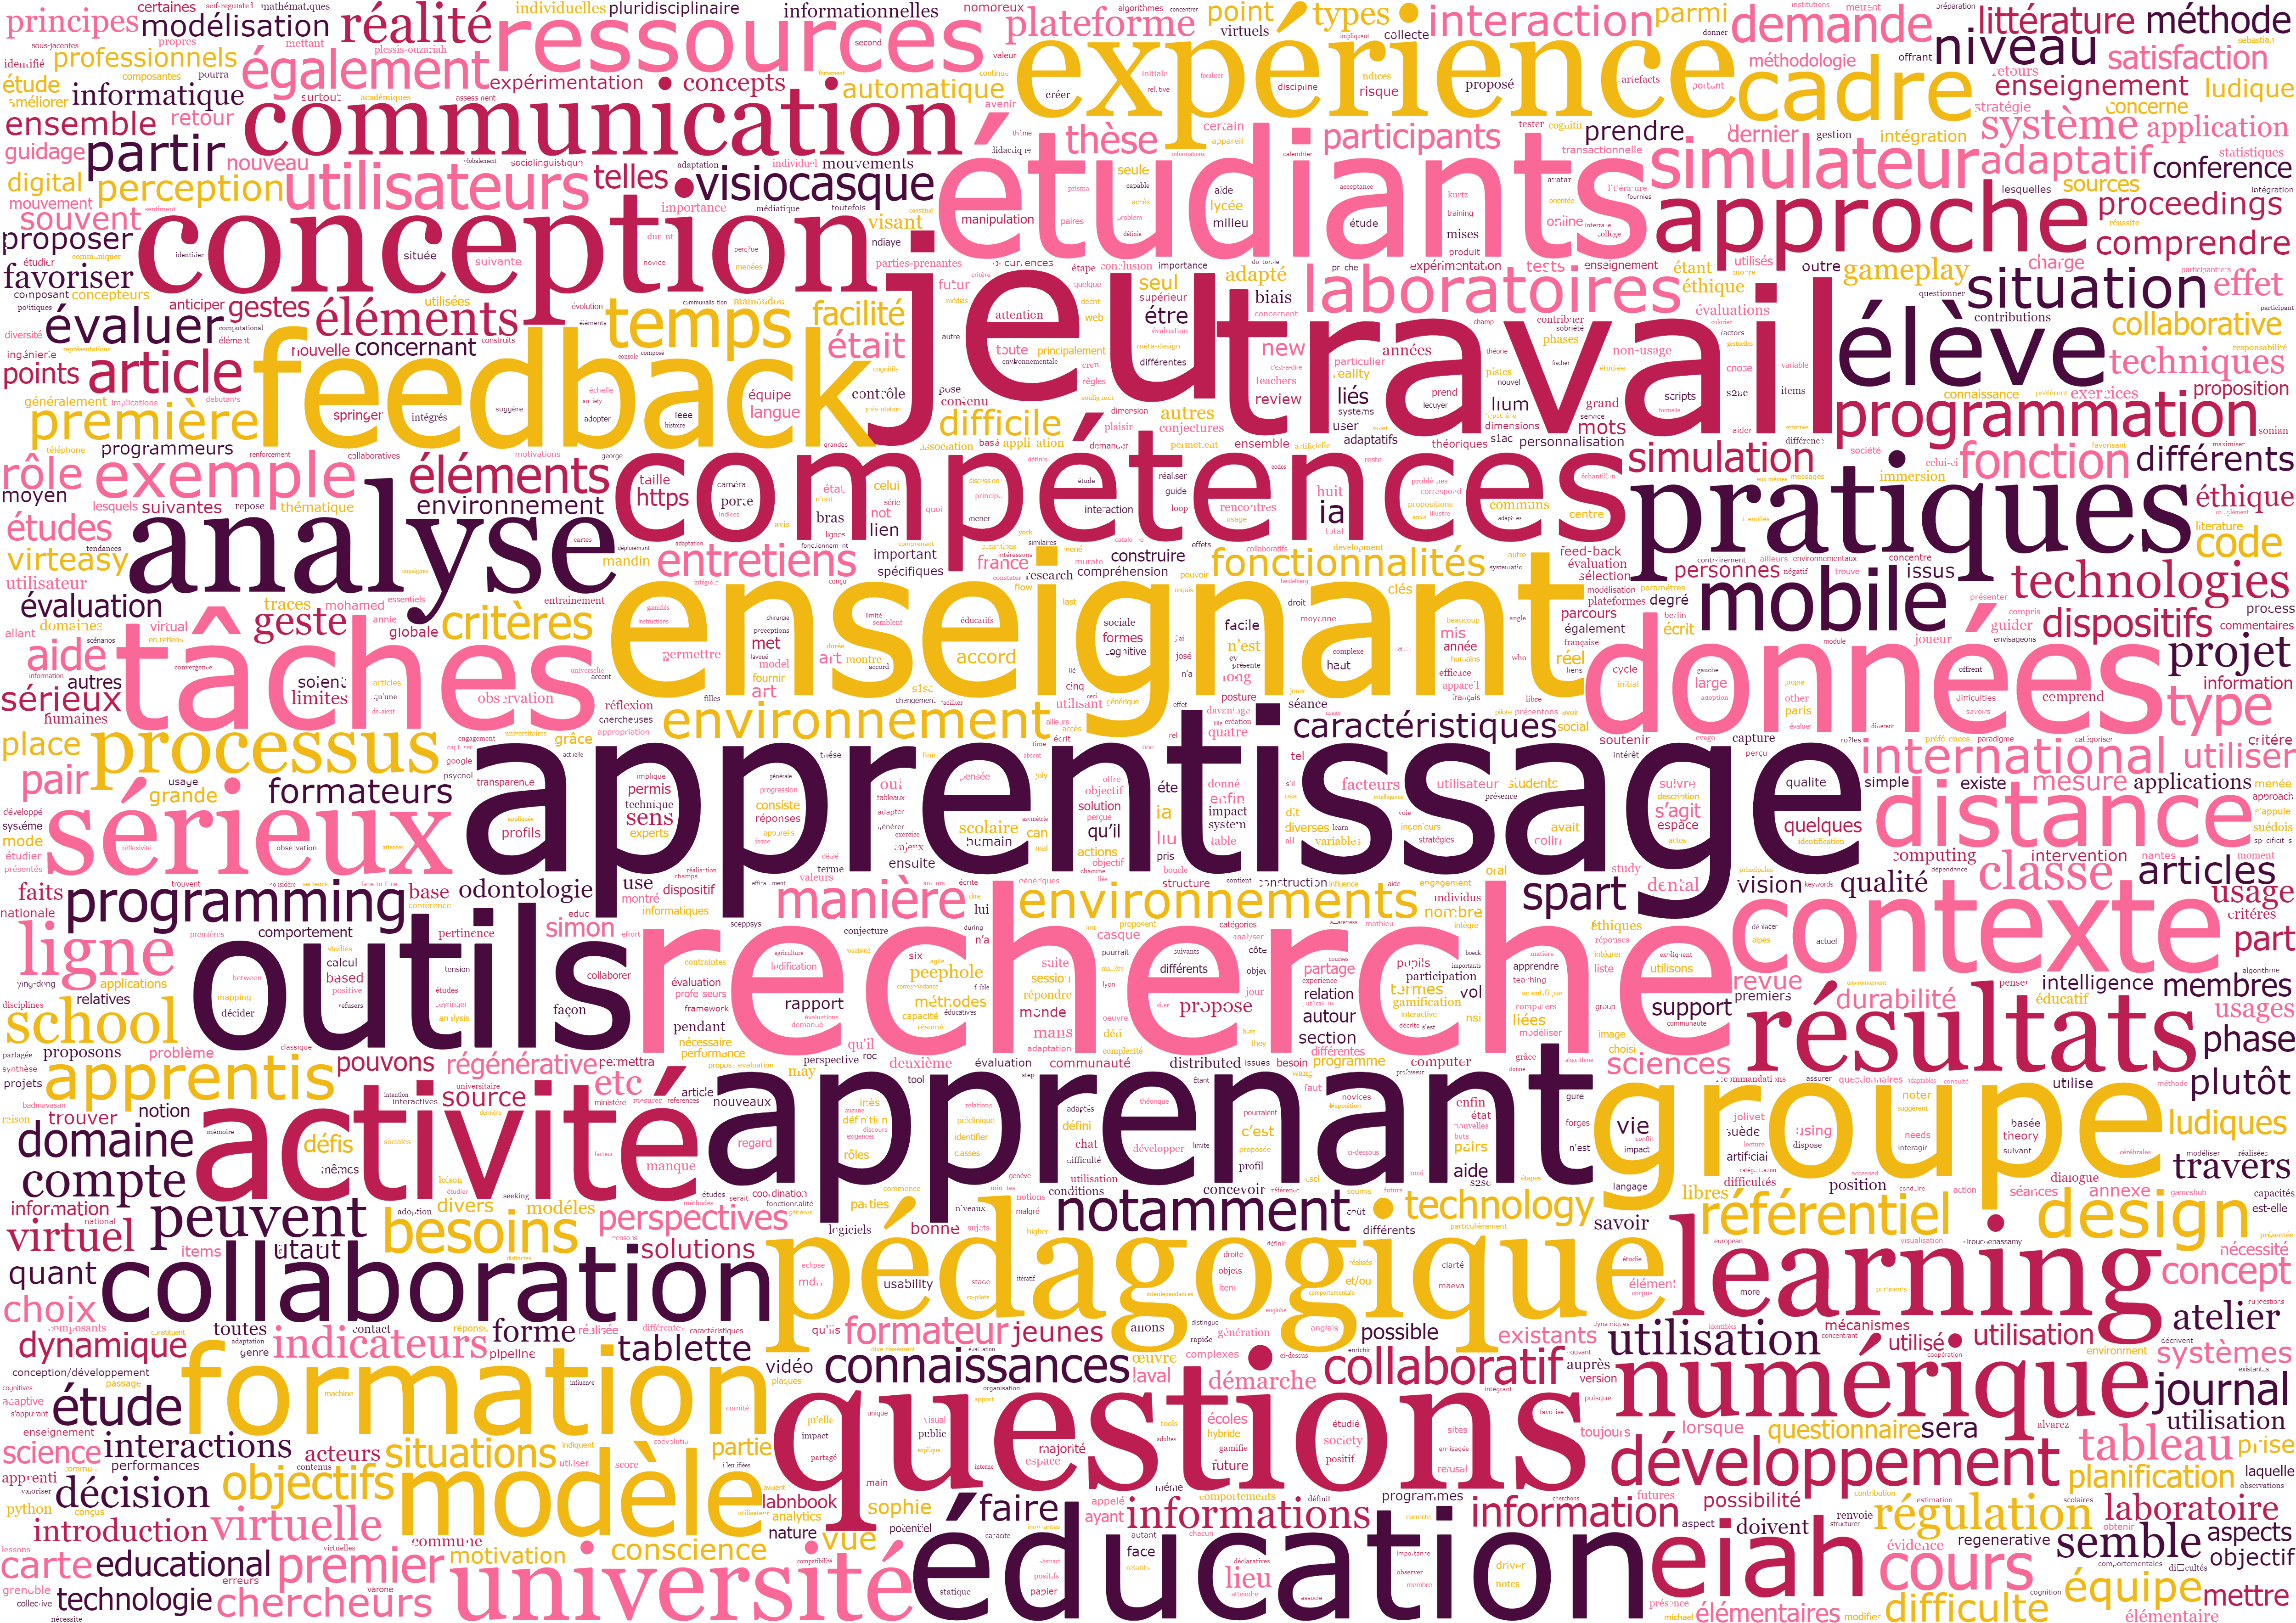
\includegraphics[width=0.8\textwidth]{Content/figures/wordcloud.png}
	\caption{Nuage de mots des contributions à RJC-EIAH 2022}
	\label{f:wordCloud}
\end{figure}

Les contributions se répartissent entre les disciplines de l’Informatique (17) et des Sciences Humaines et Sociales (13). 
Pour cette édition, 3 grandes thématiques transversales aux disciplines ont été abordées par un grand nombre des travaux présentés : les \textbf{jeux sérieu}x font l’objet d’un tiers des publications ; les \textbf{\textit{Learning Analytics}} et la fouille de données d’apprentissage sont aussi un centre d’intérêt pour plus d’un quart des publications ; enfin, la réflexion sur la \textbf{conception pédagogique} en elle-même dans le contexte des EIAH est également une thématique traitée par un cinquième des travaux. 
La figure \ref{f:wordCloud} qui expose les termes les plus présents dans les contributions fait état de ces tendances.

Ces contributions ont donc fait l’objet de cinq sessions distinctes : 
\begin{enumerate}
	\item Fouille de données d’apprentissage ;
	\item Soutien numérique à la conception pédagogique ;
	\item Conception pour les jeux sérieux ;
	\item Activités ludiques pour la collaboration ;
	\item Analytiques pour l’apprenant et l’enseignant.
\end{enumerate}

Ces rencontres jeunes chercheur.e.s ont également accueilli une conférence de la Professeur Agathe Merceron de l'Université des Sciences Appliquée de Berlin, qui porte sur la personnalisation de l’apprentissage dans l’enseignement supérieur ; aussi nous la remercions chaleureusement.

Enfin, nous remercions l’ATIEF, de même que les différents partenaires pour leur soutien à cette manifestation et plus particulièrement l’Université de Lille qui a accueillie ces rencontres au sein de son Institut Universitaire Technologique.

Pour finir, nous remercions chaleureusement tous les chercheurs en EIAH, et en particulier les jeunes chercheur·e·s sans qui ces rencontres n’auraient pas lieu.

\vspace*{2em}
\begin{flushright}
	Catherine Bonnat et Rémi Venant, co-président·e·s du comité de programme
\end{flushright}